\documentclass[sigplan, review]{acmart}

\usepackage{booktabs} % For formal tables
\usepackage{cleveref}
\usepackage{natbib}
\usepackage[utf8]{inputenc}


% Copyright
%\setcopyright{none}
%\setcopyright{acmcopyright}
%\setcopyright{acmlicensed}
\setcopyright{rightsretained}
%\setcopyright{usgov}
%\setcopyright{usgovmixed}
%\setcopyright{cagov}
%\setcopyright{cagovmixed}


% DOI
% \acmDOI{10.475/123_4}

% ISBN
% \acmISBN{123-4567-24-567/08/06}

%Conference
\acmConference[PriSC]{Workshop on Principles of Secure Compilation}{January 2018}{Los Angeles, California USA} 
\acmYear{2018}
\copyrightyear{2018}

% \acmPrice{15.00}

%\acmBadgeL[http://ctuning.org/ae/ppopp2016.html]{ae-logo}
%\acmBadgeR[http://ctuning.org/ae/ppopp2016.html]{ae-logo}


\begin{document}
\title{Enforcing Well-bracketed Control Flow and Stack Encapsulation using Linear Capabilities}
% \titlenote{Produces the permission block, and
%   copyright information}
\subtitle{Extended Abstract}
% \subtitlenote{The full version of the author's guide is available as
%   \texttt{acDat zou in dmart.pdf} document}

\author{Lau Skorstengaard}
% \orcid{}
\affiliation{%
  \institution{Aarhus University}
}
\email{lau@cs.au.dk}

\author{Dominique Devriese}
\orcid{0000-0002-3862-6856}
\affiliation{%
  \institution{imec-DistriNet, KU Leuven}
}
\email{dominique.devriese@cs.kuleuven.be}

\author{Lars Birkedal}
\affiliation{%
  \institution{Aarhus University}
}
\email{birkedal@cs.au.dk}

% The default list of authors is too long for headers}
% \renewcommand{\shortauthors}{B. Trovato et al.}


% \begin{abstract}
% This paper provides a sample of a \LaTeX\ document which conforms,
% somewhat loosely, to the formatting guidelines for
% ACM SIG Proceedings. 
% \end{abstract}

%
% The code below should be generated by the tool at
% http://dl.acm.org/ccs.cfm
% Please copy and paste the code instead of the example below. 
%
% \begin{CCSXML}
% <ccs2012>
%  <concept>
%   <concept_id>10010520.10010553.10010562</concept_id>
%   <concept_desc>Computer systems organization~Embedded systems</concept_desc>
%   <concept_significance>500</concept_significance>
%  </concept>
%  <concept>
%   <concept_id>10010520.10010575.10010755</concept_id>
%   <concept_desc>Computer systems organization~Redundancy</concept_desc>
%   <concept_significance>300</concept_significance>
%  </concept>
%  <concept>
%   <concept_id>10010520.10010553.10010554</concept_id>
%   <concept_desc>Computer systems organization~Robotics</concept_desc>
%   <concept_significance>100</concept_significance>
%  </concept>
%  <concept>
%   <concept_id>10003033.10003083.10003095</concept_id>
%   <concept_desc>Networks~Network reliability</concept_desc>
%   <concept_significance>100</concept_significance>
%  </concept>
% </ccs2012>  
% \end{CCSXML}

% \ccsdesc[500]{Computer systems organization~Embedded systems}
% \ccsdesc[300]{Computer systems organization~Redundancy}
% \ccsdesc{Computer systems organization~Robotics}
% \ccsdesc[100]{Networks~Network reliability}


% \keywords{ACM proceedings, \LaTeX, text tagging}

% \begin{teaserfigure}
%   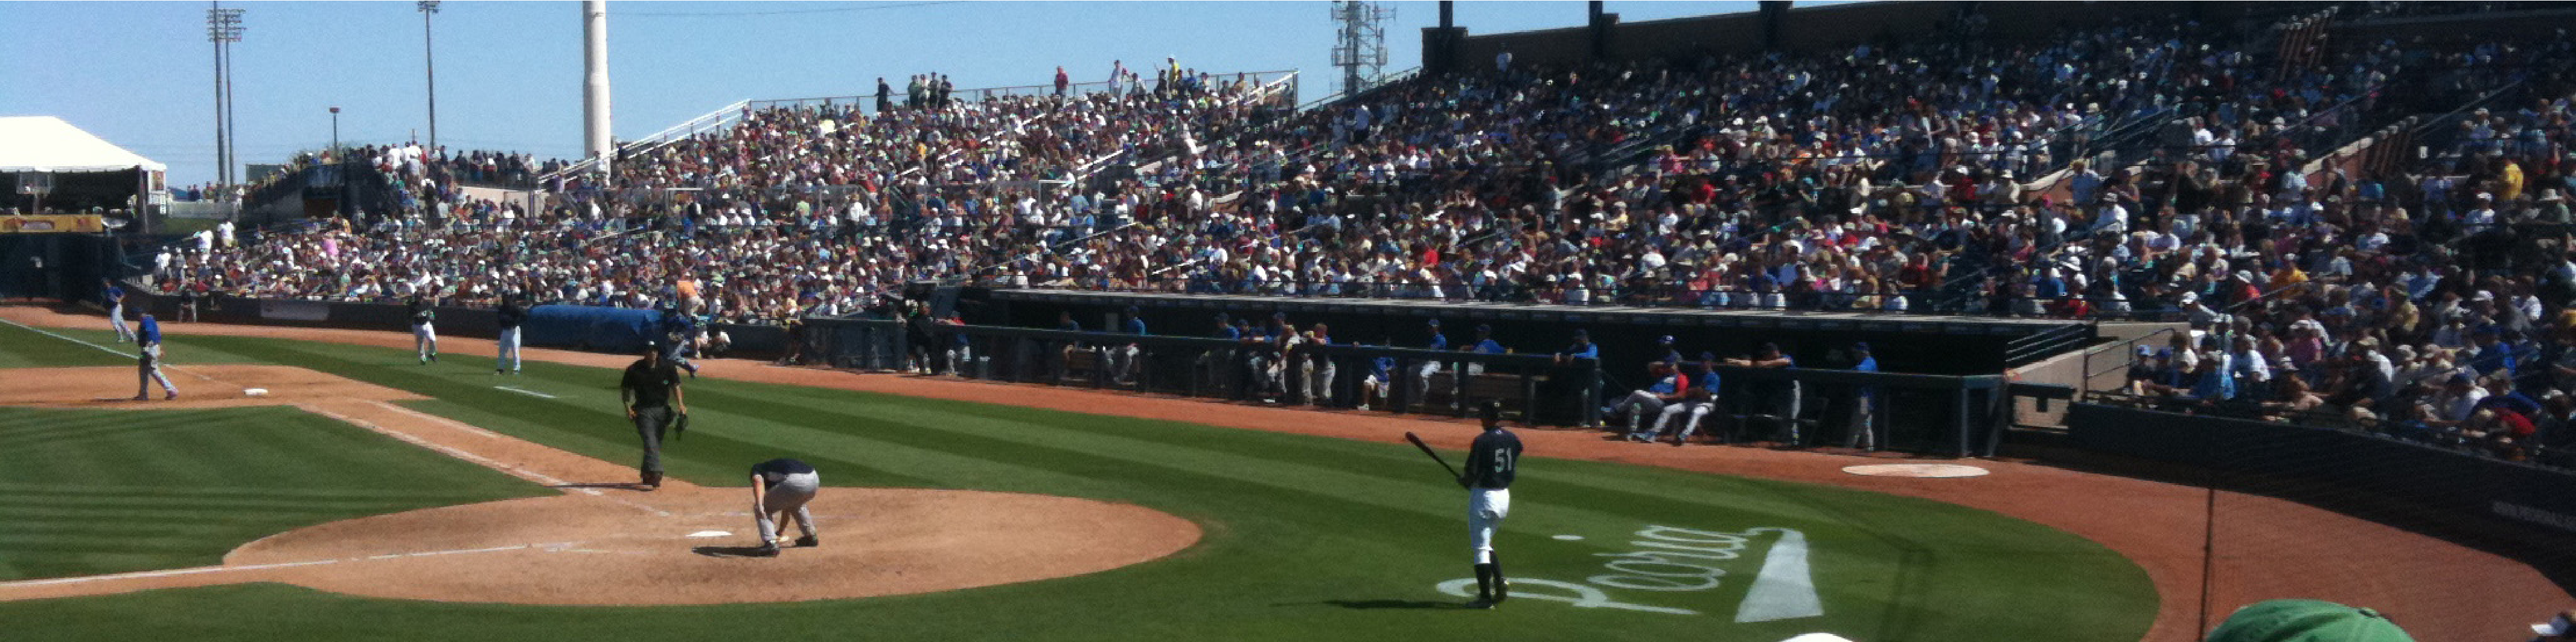
\includegraphics[width=\textwidth]{sampleteaser}
%   \caption{This is a teaser}
%   \label{fig:teaser}
% \end{teaserfigure}


\maketitle

\section{Introduction}
Secure compilers preserve source-language (security-relevant) properties even when the  compiled code interacts with arbitrary target-language components.
Generally, properties that hold in the source language but not in the target language, need to be somehow enforced by the compiler.
Two properties that hold in many high-level source languages, but not in the assembly languages that they are compiled to are the well-bracketedness of control flow and the encapsulation of local state.

Well-bracketed control flow expresses that invoked functions must either return to their callers, invoke other functions themselves or diverge, and generally holds in programming languages that do not offer a primitive form of continuations. 
At the assembly level, this is not so obvious, as invoked functions get direct access to return pointers, that they are supposed to jump to a single time, at the end of their execution, but there is no guarantee that untrusted assembly code respects this intended usage.
Particularly, it may invoke return pointers from other stack frames than the one it was invoked from, either ones from frames higher in the call stack or from stack frames that no longer exist because they have already been returned to before. 

Local state encapsulation is the guarantee that when a function invokes another function, its local variables will not have been modified when the invoked function returns.
At the assembly level, this property is also far from obvious, local variables are stored on the stack when another function is invoked, and functions are not supposed to touch stack frames other than their own.
However, untrusted assembly code is usually not prevented from ignoring this requirement and overwriting the local state of its caller or other stack frames.

To enforce these properties, a target language is needed with some form of security primitive that can be used to prevent untrusted code from misbehaving, without imposing too much overhead on well-behaved code.
The virtual-memory based security primitives on commodity processors do not seem sufficiently fine-grained to efficiently support this type of enforcement.
More suitable security primitives are offered by a type of processors known as capability machines \citep{levy_capability-based_1984,watson_cheri:_2015}.
These processors use tagged memory to enforce a strict separation between integers and \emph{capabilities}: pointers that carry authority.
Capabilities come in different flavours.
Memory capabilities are used to read and write to memory.
Additionally, CHERI offers a notion of sealed code-data pairs of capabilities that represent a type of encapsulated closure: a piece of code coupled with private state that it gains access to upon invocation.\footnote{Other capability machines offer other mechanisms that can be used to the same effect.} 

CheriBSD, an operating sytem built on the CHERI capability machine, uses per-component separate stacks and a central, trusted stack manager component to enforce well-bracketed control flow and private state encapsulation \citep{watson_cheri:_2015}.
To prevent the stack pointer (or derivatives from it) from being passed to other components, CheriBSD uses local capabilities: a type of capabilities that can be kept in registers but not stored in memory (except through store-local capabilities like the stack pointer itself).
The literature does not contain many details about the mechanism, let alone a formal analysis, but most importantly, the mechanism does not seem like it can support higher-order interfaces (e.g. C function pointers) in a scalable fashion.

In recent work, we have been looking at an alternative approach \citep{skorstengaard_reasoning_2017}.
It is also based on CHERI's local capabilities, but combines them with a more traditional, single, shared stack that scales better in the presence of higher-order interfaces.
By passing stack and return pointers as local capabilities, our mechanism effectively prevents callees from storing them on the heap.
Using a step-indexed Kripke logical relation, we are able to prove correctness of programs that rely on well-bracketed control flow in a complex way.

While this approach works quite well, this paper investigates another alternative approach.
The aim of this new approach is to resolve two limitations: (1) the need to clear the stack on boundary crossings and (2) the lack of a formal statement of well-bracketed control flow and local state encapsulation.
In the next two sections, we discuss these two limitations and how we intend to resolve them.

\section{Linear Capabilities, not Local}
What we essentially want to achieve in a secure calling convention is to give an invoked function access to a stack pointer and a return pointer, but only temporarily: during the execution of the invoked function. 
In our original approach, we make both pointers local, so that the CHERI processor guarantees, essentially, that they can only be stored in registers or on the stack.
To make sure that an invoked function has no way of transferring the pointers accross outside the lifetime of its stack frame, it then suffices to block only these two communication channels, rather than the entire memory.
In other words, our approach relies on clearing registers and the stack before we pass control to untrusted code, as a way of preventing it from obtaining access to other stack and return pointers than the ones for the stack frame it is invoked in.
The requirement for clearing registers is unproblematic, but clearing the entire stack upon every boundary crossing is a non-trivial requirement.
We speculate that it can be made efficient with custom hardware extensions\footnote{Specifically, we imagine a kind of pre-L0 processor cache that does not retain values but only remembers that a certain range has been zeroed out.}, but this is not obvious.

An alternative that does not have this requirement, relies on \emph{linear capabilities}, rather than local ones.
Linear capabilities are (to the best of our knowledge) a new concept, similar to CHERI's local capabilities.\footnote{One author of this abstract is also investigating linear capabilities in another application, also submitted to PriSC.}
The idea is that all capabilities are marked as either regular or linear.
When they are linear, they are subject to special restrictions, enforced by the hardware, that prevent them from being duplicated.
When linear capabilities are moved to a new location in registers or memory, they are erased from their old location.
A few special instructions are needed to make this workable, e.g.\ a split instruction that splits a memory capability for a region of memory into disjoint capabilities for two parts of the region and a splice instruction that performs the reverse.
Linearity of a capability is a powerful tool: when we pass a linear capability to untrusted code and we receive the same capability back, we can be sure that they will not have been able to store a copy of it.
Similarly, if we receive a linear capability from untrusted code and we know that the capability addresses memory that is only ever addressed by linear capabilities, then we are sure that the untrusted code can no longer access that memory.

As such, linear capabilities can be used as an alternative to local capabilities to enforce well-bracketed control flow.
We cannot provide full details here for space reasons, but the idea is essentially the following.
By passing stack and return pointers as linear capabilities, and requiring that invoked functions hand in their stack pointer upon return, untrusted code are prevented from keeping hold of old stack and return pointers past their intended lifetime, essentially because they can only ever have one copy that they have to hand in when this lifetime ends.

\section{Formalising well-bracketed control flow}
The second improvement we are making is related to the properties of well-bracketed control flow and local state encapsulation.
Our previous work did not actually have a precise statement of these properties.
We only show a reasoning technique that can be used to prove certain example programs that rely on the properties.
Although it can be argued that this proof technique should perhaps qualify as a formal statement of the properties, we are investigating an alternative approach, based on the notion of fully abstract compilation \citep{abadi_protection_1999}.

We intend to start from a formalisation of an assembly language for a capability machine with linear capabilities (the target language).
Our idea is then to introduce a variant of this target language that features a primitive stack, built into the operational semantics, as well as additional instructions like call and return.
While the original target language is a standard assembly language without even the notion of a stack, this variant language (the source language) does have a stack, and control flow well-bracketedness and local state encapsulation are evident properties of the operational semantics.
We can formalise our calling convention in the definition of a compiler from the source language to the target language.
Additionally, we conjecture that this compiler can be proved fully abstract, thus formally expressing and establishing security of the calling convention.

Interestingly, the proof of full abstraction for this compiler is expected to use a very simple back-translation, that simply maps every target language instruction to the corresponding instruction in the source.
This back-translation works because we construct our source language in such a way that it has direct counterparts to every target language value.
Specifically, the source language contains a representation of stack and return pointers as unspecified abstract values whose behavior corresponds to their target counterparts, but in a way that guarantees the intended properties of well-bracketed control flow and local state encapsulation.

\bibliographystyle{ACM-Reference-Format}
\bibliography{references} 

\end{document}
